\documentclass{article}

% math, graphics, and formatting
\usepackage{amsmath,amsbsy,amssymb,amsthm,fullpage,graphicx,pgfplots,breqn}
\usepackage{verbatim,mathtools}

% physics
\usepackage{physics}
\newcommand{\h}{\hbar}
\renewcommand{\vec}{\mathbf}

% Times New Roman
\usepackage{newtxtext}
\usepackage{newtxmath}
\renewcommand{\mathbb}{\varmathbb}
%\usepackage{libertine}
%\usepackage[libertine]{newtxmath}

% section numbering: e.g. 2b (ii)
\renewcommand\thesection{\arabic{section}}
\renewcommand\thesubsection{\thesection\alph{subsection}}
\renewcommand\thesubsubsection{\thesubsection\,(\roman{subsubsection})}

% theorems & proofs
\theoremstyle{definition}
\newtheorem*{prop}{Claim}
\newtheorem*{claim}{Claim}
\newtheorem*{prob}{Problem}
\newtheorem*{obs}{Observation}
\newtheorem*{lemma}{Lemma}
\newtheorem*{thm}{Theorem}
\newtheorem*{disc}{Discussion}
\newtheorem*{defn}{Definition}
\newtheorem*{eg}{Example}

% derivatives
\newcommand{\pp}{\partial}
\newcommand{\pd}[2]{\ensuremath\frac{\pp #1}{\pp #2}}
\newcommand{\pdd}[2]{\ensuremath\frac{\pp^2 #1}{\pp #2^2}}
\renewcommand{\dd}[2]{\ensuremath\frac{d#1}{d#2}}
\newcommand{\ddd}[2]{\ensuremath\frac{d^2 #1}{d #2^2}}
\newcommand{\del}{\nabla}

% sets and complex numbers
\newcommand{\R}{\mathbb R}
\renewcommand{\Re}{\textrm{Re}}
\renewcommand{\Im}{\textrm{Im}}
%\renewcommand{\bar}{\overline}
\newcommand{\nin}{\not\in}
\newcommand{\str}[1]{\ensuremath{\langle #1 \rangle}}

% probability and stats
\renewcommand{\var}{\ensuremath\mathbf{Var}}
\newcommand{\E}{\ensuremath\mathbf{E}}
\renewcommand{\P}{\ensuremath\mathbf{P}}

% measurement
\newcommand{\un}[1]{\;\mathrm{#1}}
\newcommand{\ch}[1]{\mathrm{#1}}

% Greek letters are hard
\newcommand{\ep}{\varepsilon}
\newcommand{\om}{\omega}

% formatting
\renewcommand{\sp}[1]{\;\;\;\text{ #1 }\;\;\;}
\newcommand{\cc}{\texttt}
\newcommand{\plop}[2]{
    \begin{figure}\centering
        \includegraphics[width=0.8\textwidth]{#1}
        \caption{\label{#1}#2}
    \end{figure}
}
\newcommand{\sbsplop}[4]{
    \begin{figure}\centering
        \includegraphics[width=0.49\textwidth]{#1}
        \includegraphics[width=0.49\textwidth]{#2}
        \caption{\label{#1}#3}
        {#4}
    \end{figure}
}

\usepackage{fancyhdr}
\usepackage[margin=1in, headheight=50pt]{geometry}
\pagestyle{fancy}
\lhead{\textbf{Ph21 Set 4}}
\chead{}
\rhead{Aritra Biswas}
\setlength{\headsep}{20pt}

\begin{document}

\begin{thm}[Bayes' Theorem]
The probability that a system is well-described a model with
parameter set $\vec X$, given a dataset $\vec D$ and initial knowledge
$I$, is:
\begin{align*}
\Pr(\vec X | \vec D, I) =
{
    \Pr(\vec D | X, I) \cdot \Pr(\vec X | I)
    \over
    \Pr(\vec D | I)
}.
\end{align*}
$\Pr(\vec X | I)$ is called the \emph{prior}, $\Pr(\vec X | \vec D, I)$
the \emph{posterior}, and $\Pr(\vec D | \vec X, I)$ the \emph{likelihood}.
\end{thm}

\section{Coin tossing}

We consider a sequence of tosses of a biased coin. The coin can be
modeled with a single parameter $H \in [0, 1]$, the probability of
heads on a single toss. Thus our parameter set is $\vec X = \{ H \}$.

The dataset $\vec D$ can be reduced to a tuple $(n, h)$ where $h$
is the number of heads in $n$ tosses. There is no other
prior information: $I = \emptyset$. The probability of obtaining
some data given the parameter $H$ is:
\begin{align*}
\Pr(\vec D | \vec X, I) = \Pr\Big( (n, h) | H \Big)
= {n \choose h} H^h (1 - H)^{n - h},
\end{align*}
since there are ${n \choose h}$ ways of getting $h$ heads (each
with probability $H$) and $n - h$ tails (each with probability
$1 - H$).

In this simulation, we choose $H = 0.38$ and three prior distributions:
an uniform one, a Gaussian with $\sigma = 0.1$ centered around $\mu = 0.5$,
representing a belief that the coin is fair, and a Gaussian
with $\sigma = 0.05$ centered around $\mu = 0.5$, representing a stronger
belief that the coin is fair. Results for each prior are shown
in Figures 1-3.

\plop{coin_uniform.pdf}{Likelihoods for multiple $n$ with an
uniform prior.}
\plop{coin_widegauss.pdf}{Likelihoods for multiple $n$ with an
wide Gaussian prior.}
\plop{coin_narrowgauss.pdf}{Likelihoods for multiple $n$ with
a narrow Gaussian prior.}

\section{Lighthouse problem}

We have a lighthouse at a distance $\beta$ from the shore and
at a location $\alpha$ along the shore. The lighthouse emits
flashes at random angles $\theta_k$ which arrive at the shore
at locations $x_k$.
Let:
\begin{align*}
f_\theta(\theta) &\equiv \Pr(\theta_k = \theta) \;\text{be the
pdf of $\theta_k$,} \\
F_\theta(\theta) &\equiv \Pr(\theta_k \le \theta) \;\text{be the
cdf of $\theta_k$,} \\
f_x(x) &\equiv \Pr(x_k = x) \;\text{be the
pdf of $x_k$,} \\
F_x(x) &\equiv \Pr(x_k \le x) \;\text{be the
cdf of $x_k$.}
\end{align*}

Since the lighthouse emits flashes at random angles, we assume
$\theta_k$ is uniformly distributed:
\begin{align*}
f_\theta(\theta) = {1 \over 2\pi},
\sp{}
F_\theta(\theta) = \int_0^\theta f_\theta(\tilde\theta) \, d\tilde\theta
= {\theta \over 2\pi}.
\end{align*}
To derive $f_x$, we first derive $F_x$:
\begin{align*}
F_x(x) = \Pr(x_k \le x) = \Pr(\theta_k \le \hat\theta(x)) =
F_\theta\Big(\hat\theta(x)\Big),
\end{align*}
where $\hat\theta(x)$ is the angle that creates a flash at $x$. To find it,
we use the geometry of the problem:
\begin{align*}
\hat\theta(x) &= \arctan\left(x - \alpha \over \beta\right).
\end{align*}
Thus:
\begin{align*}
F_x(x) &= {1 \over 2\pi} \arctan\left(x - \alpha \over \beta\right).
\\
f_x(x) &= \dd{}{x} F_x(x) = {\beta / 2\pi \over (x - \alpha)^2 + \beta^2}.
\end{align*}
This makes intuitive sense: the distribution is a Lorentzian centered
around $\alpha$, the location of the the lighthouse along the shore. The
further the lighthouse is, the wider the distribution is.

For our study we choose $\alpha = 1.0$ and $\beta = 1.5$.
We again use three prior distributions: an uniform one, a wide Gaussian
centered at $\mu = 1.5$ with $\sigma = 0.3$, and a narrow Gaussian with
$\mu = 1.5$ with $\sigma = 0.1$.

Results for the one-dimensional case, where $\beta$ is known but $\alpha$
is not, are shown in Figures 4-6.

\plop{lh1d_uniform.pdf}{Likelihoods for multiple $n$ with an
uniform prior.}
\plop{lh1d_widegauss.pdf}{Likelihoods for multiple $n$ with a
wide Gaussian prior.}
\plop{lh1d_narrowgauss.pdf}{Likelihoods for multiple $n$ with a narrow
Gaussian prior.}

In the two-dimensional case, we use identical priors for each parameter.
Results are shown in Figures 7-9.

\begin{figure}\centering
    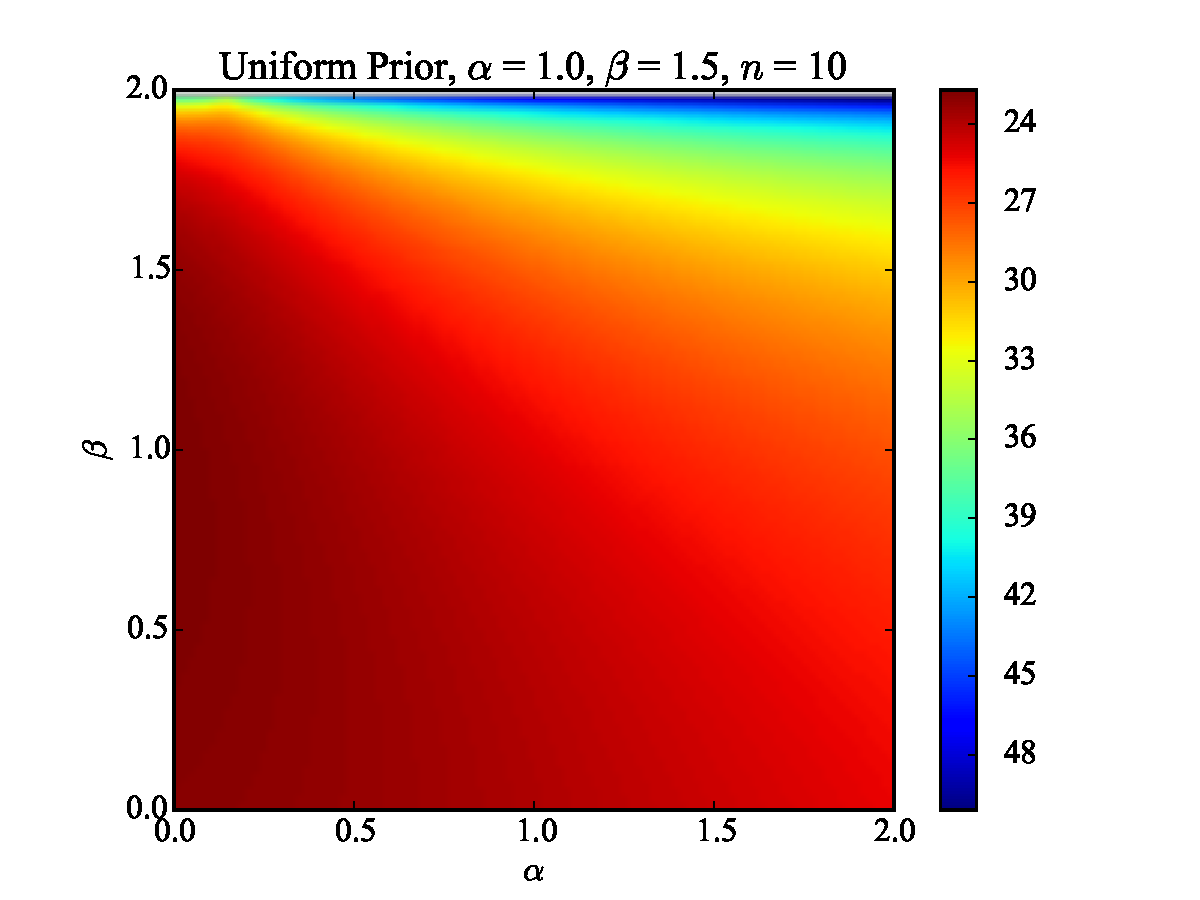
\includegraphics[width=0.49\textwidth]{lh2d_1.pdf}
    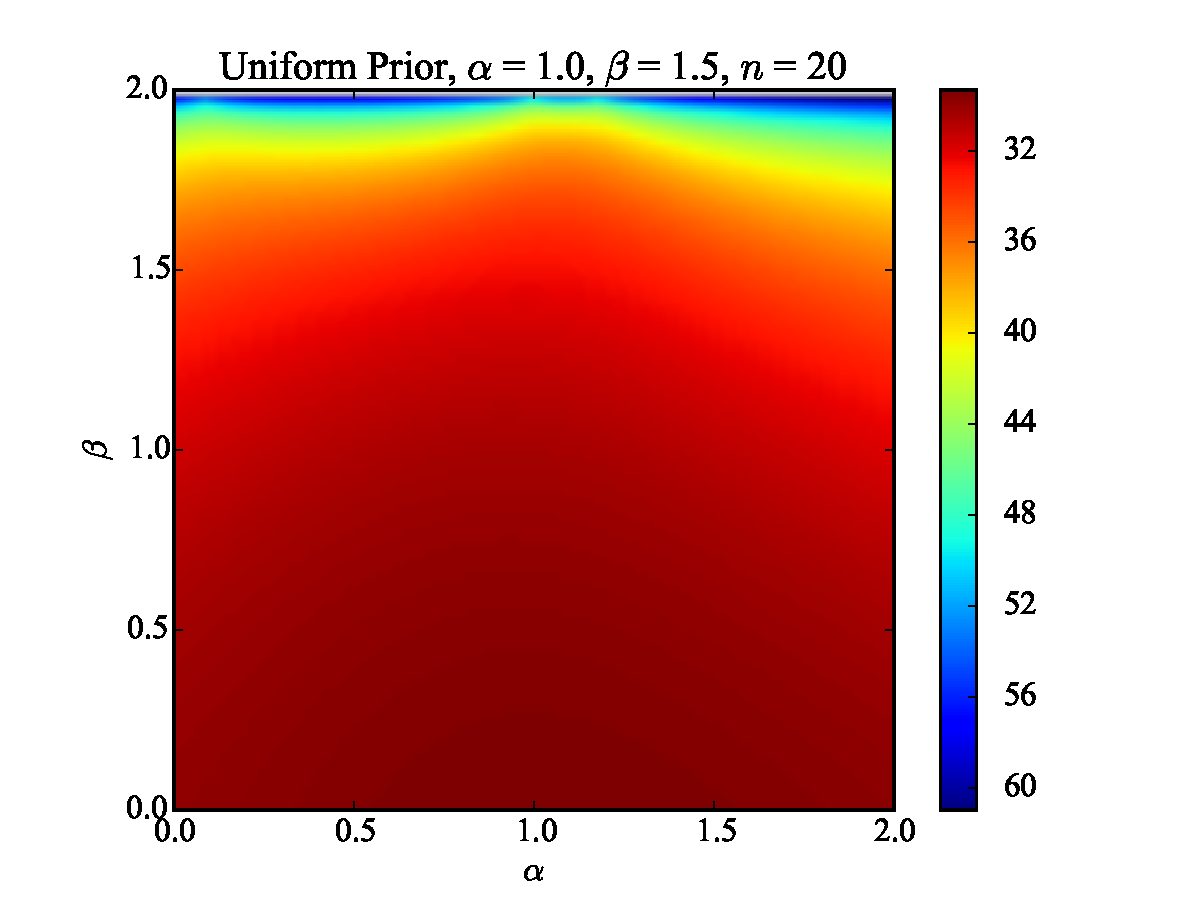
\includegraphics[width=0.49\textwidth]{lh2d_2.pdf}
    \\
    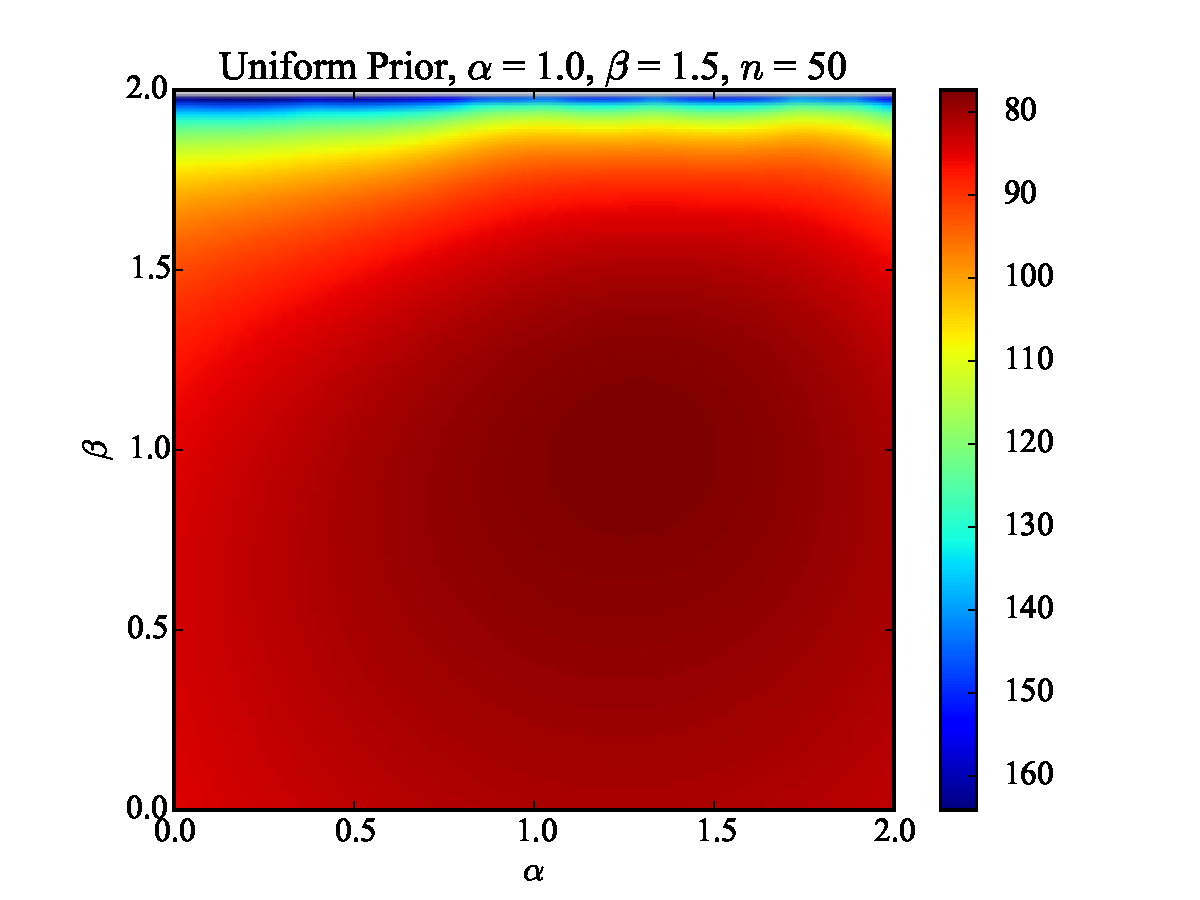
\includegraphics[width=0.49\textwidth]{lh2d_3.pdf}
    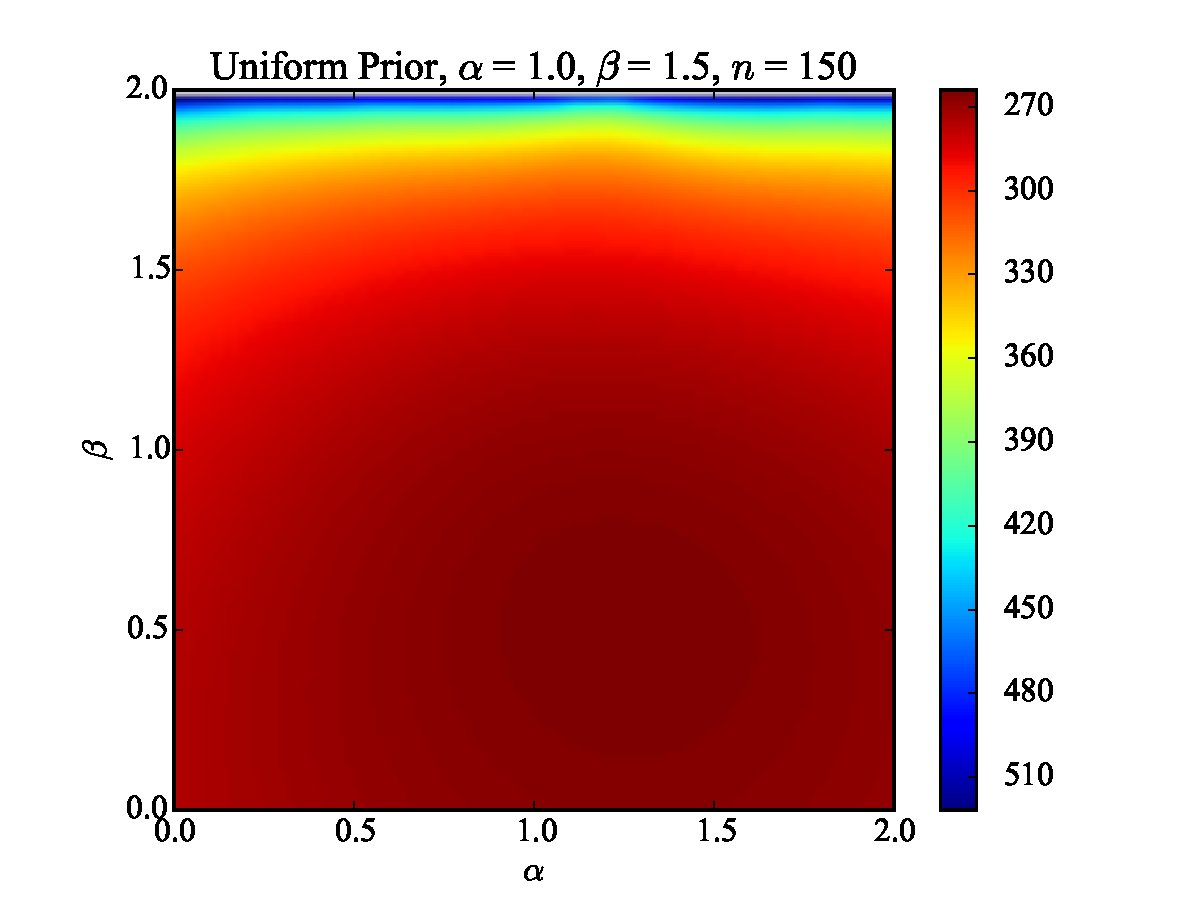
\includegraphics[width=0.49\textwidth]{lh2d_4.pdf}
    \caption{\label{2d_uniform}Likelihoods for multiple $n$ with an uniform
    prior.}
\end{figure}

\begin{figure}\centering
    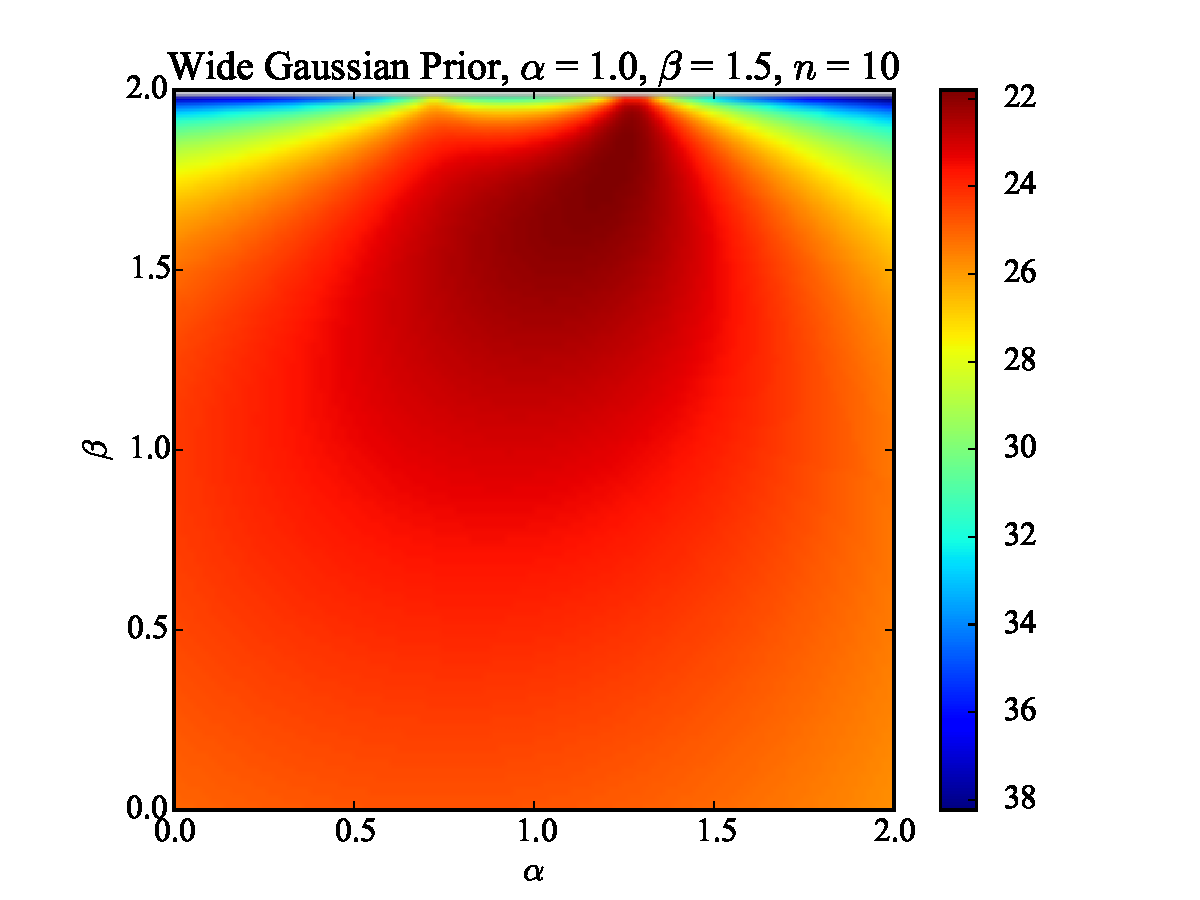
\includegraphics[width=0.49\textwidth]{lh2d_5.pdf}
    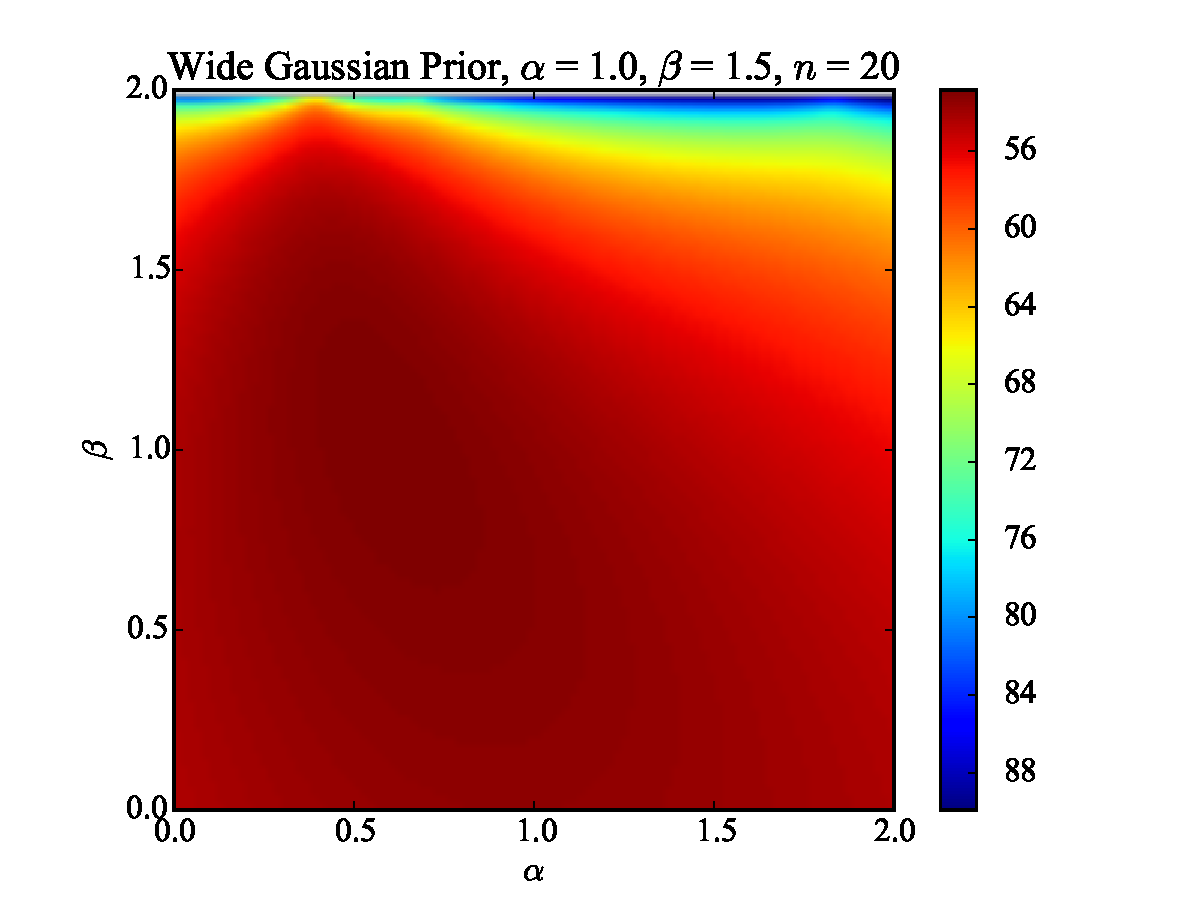
\includegraphics[width=0.49\textwidth]{lh2d_6.pdf}
    \\
    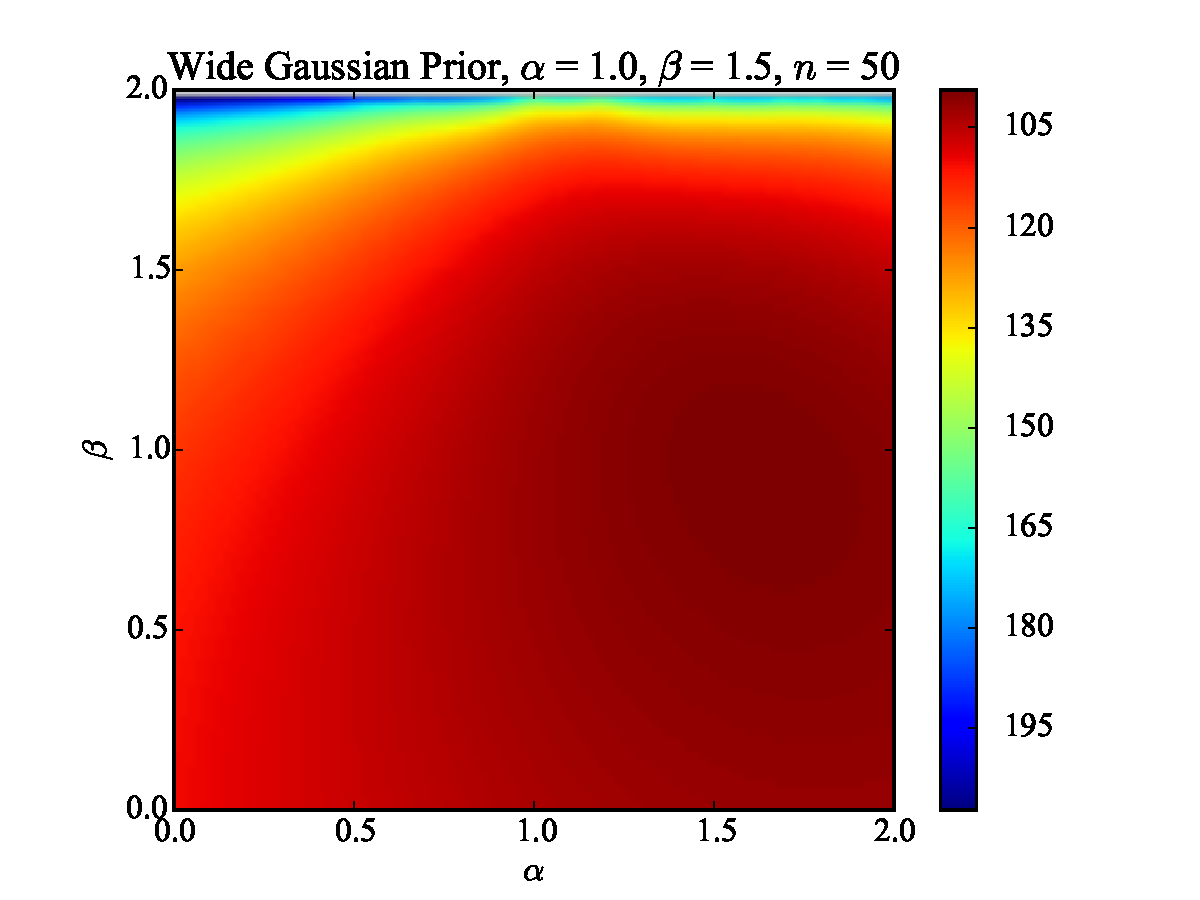
\includegraphics[width=0.49\textwidth]{lh2d_7.pdf}
    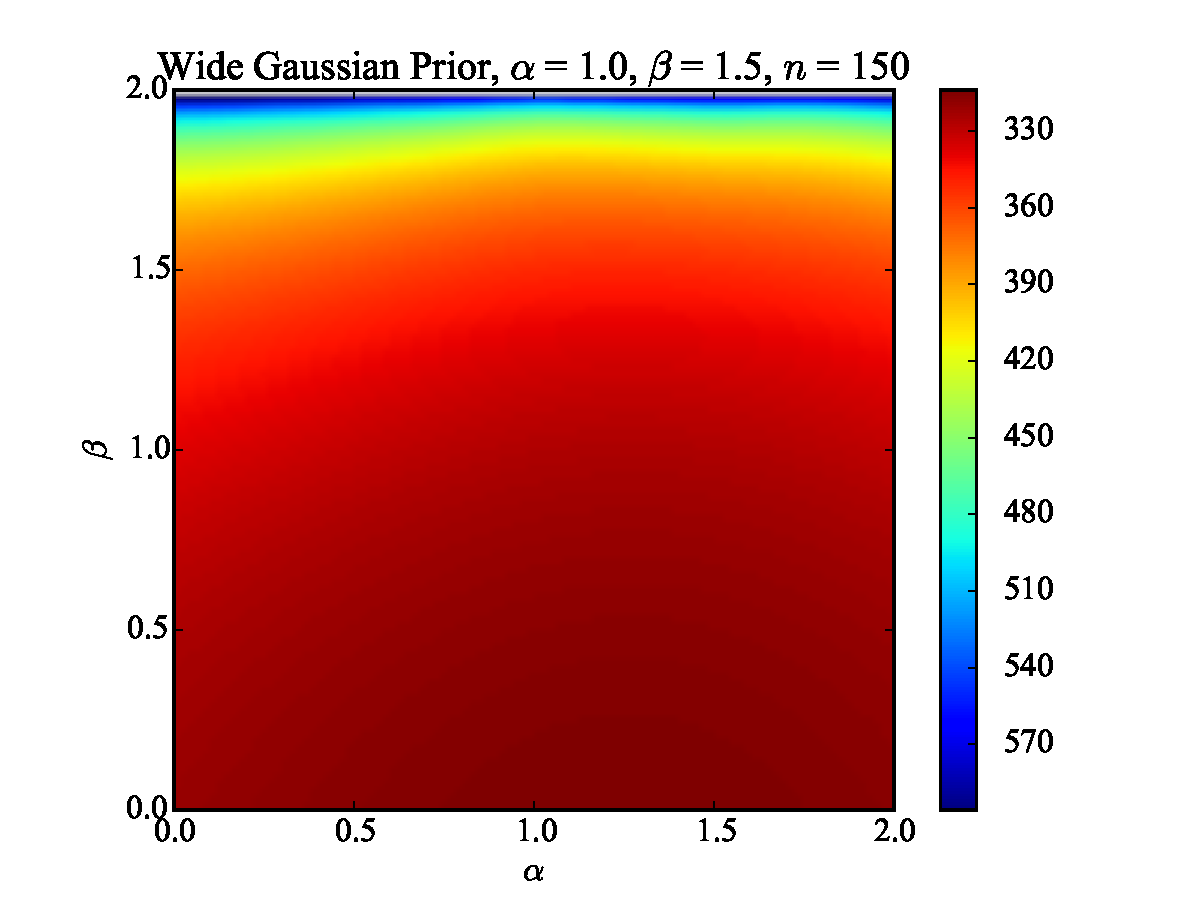
\includegraphics[width=0.49\textwidth]{lh2d_8.pdf}
    \caption{\label{2d_widegauss}Likelihoods for multiple $n$ with a wide
    Gaussian prior.}
\end{figure}

\begin{figure}\centering
    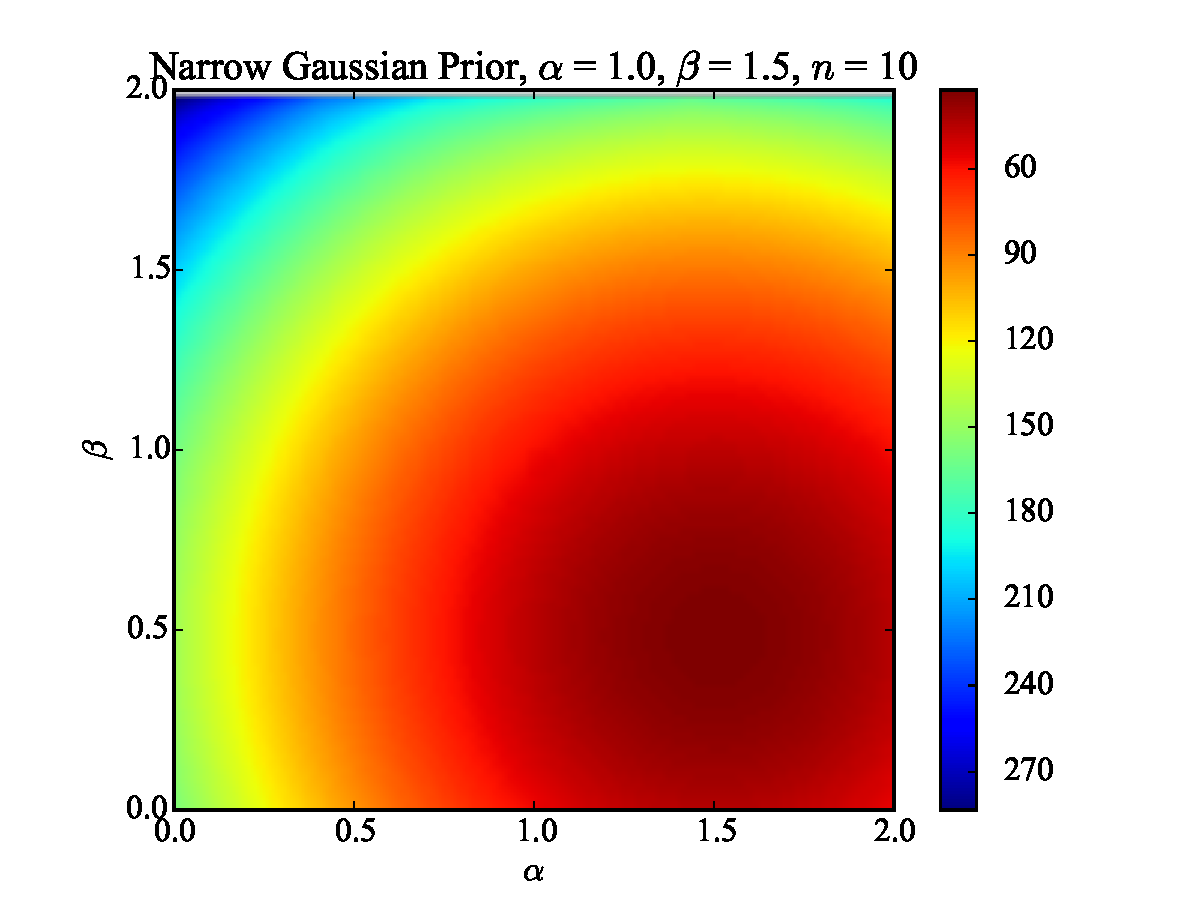
\includegraphics[width=0.49\textwidth]{lh2d_9.pdf}
    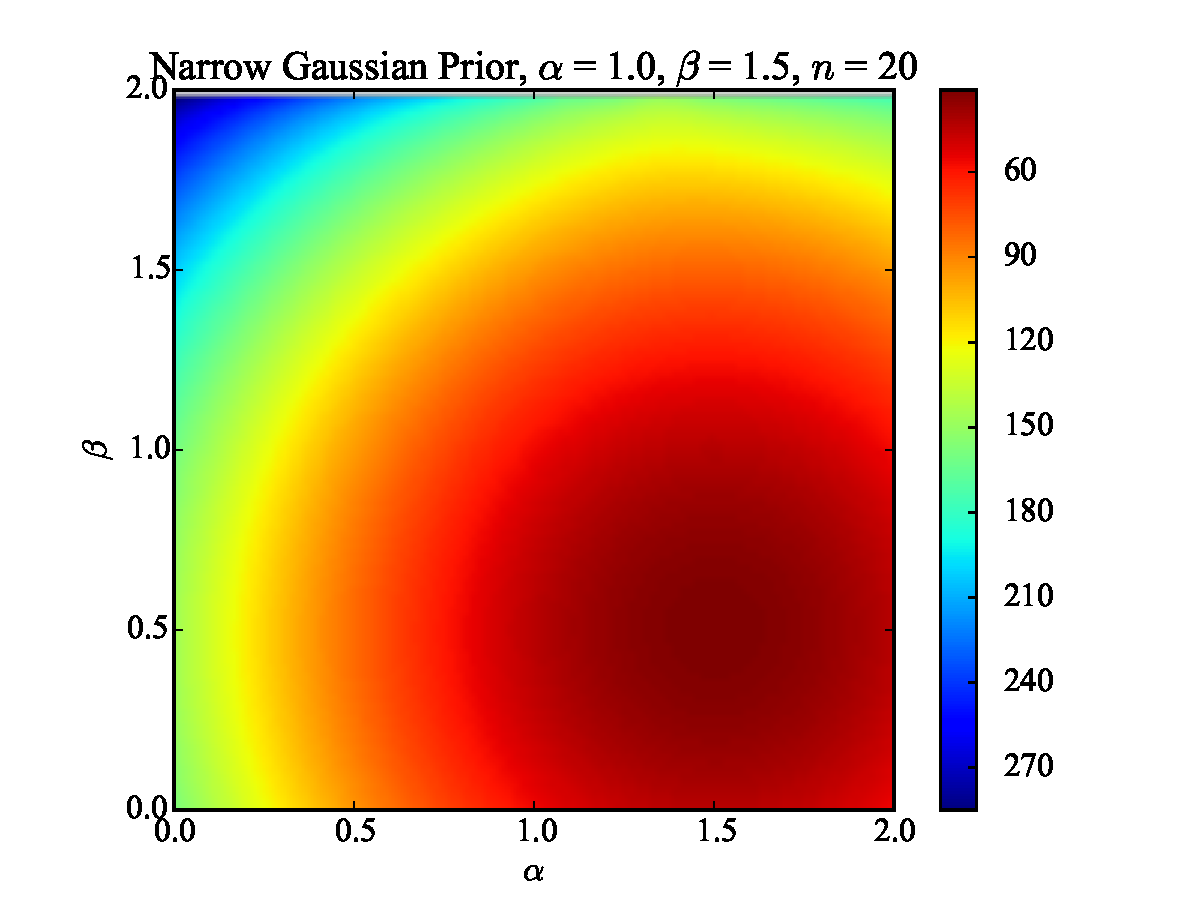
\includegraphics[width=0.49\textwidth]{lh2d_10.pdf}
    \\
    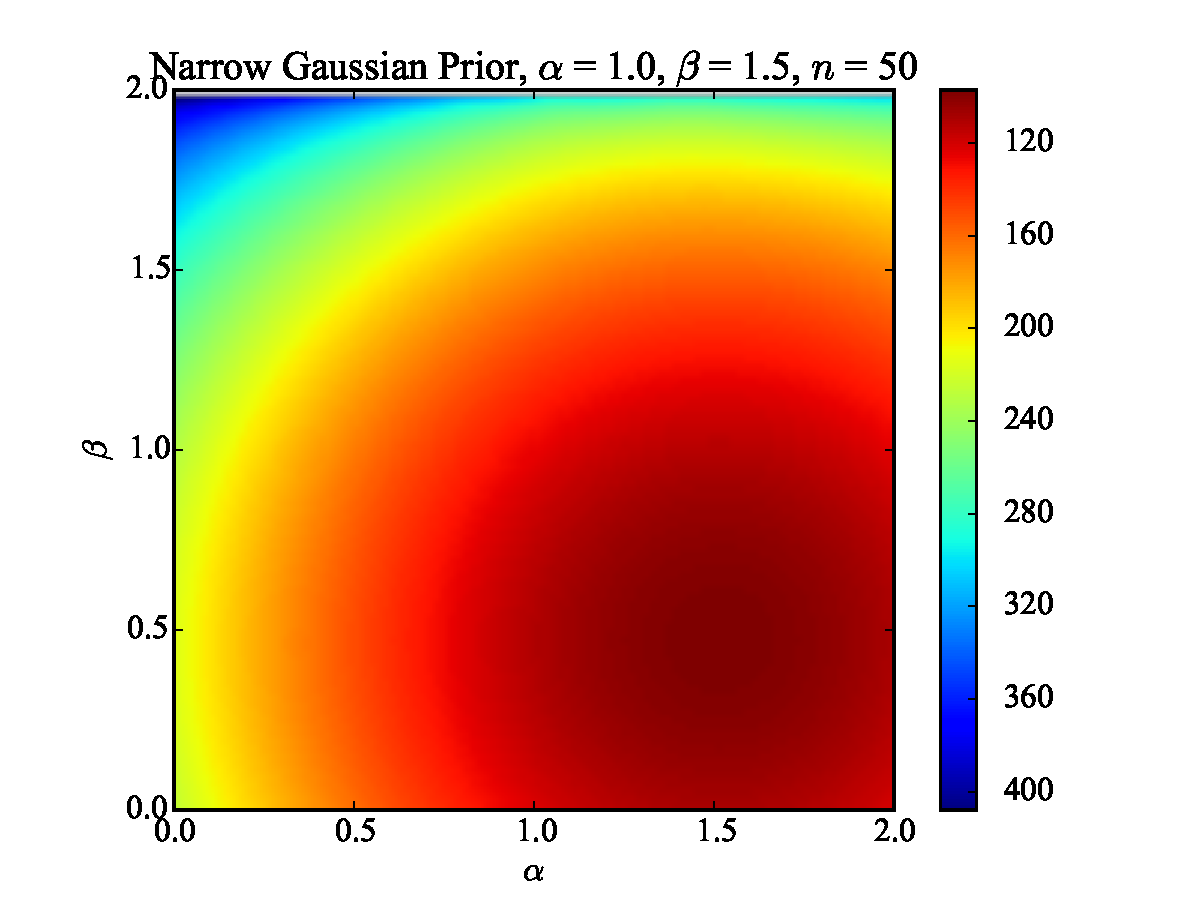
\includegraphics[width=0.49\textwidth]{lh2d_11.pdf}
    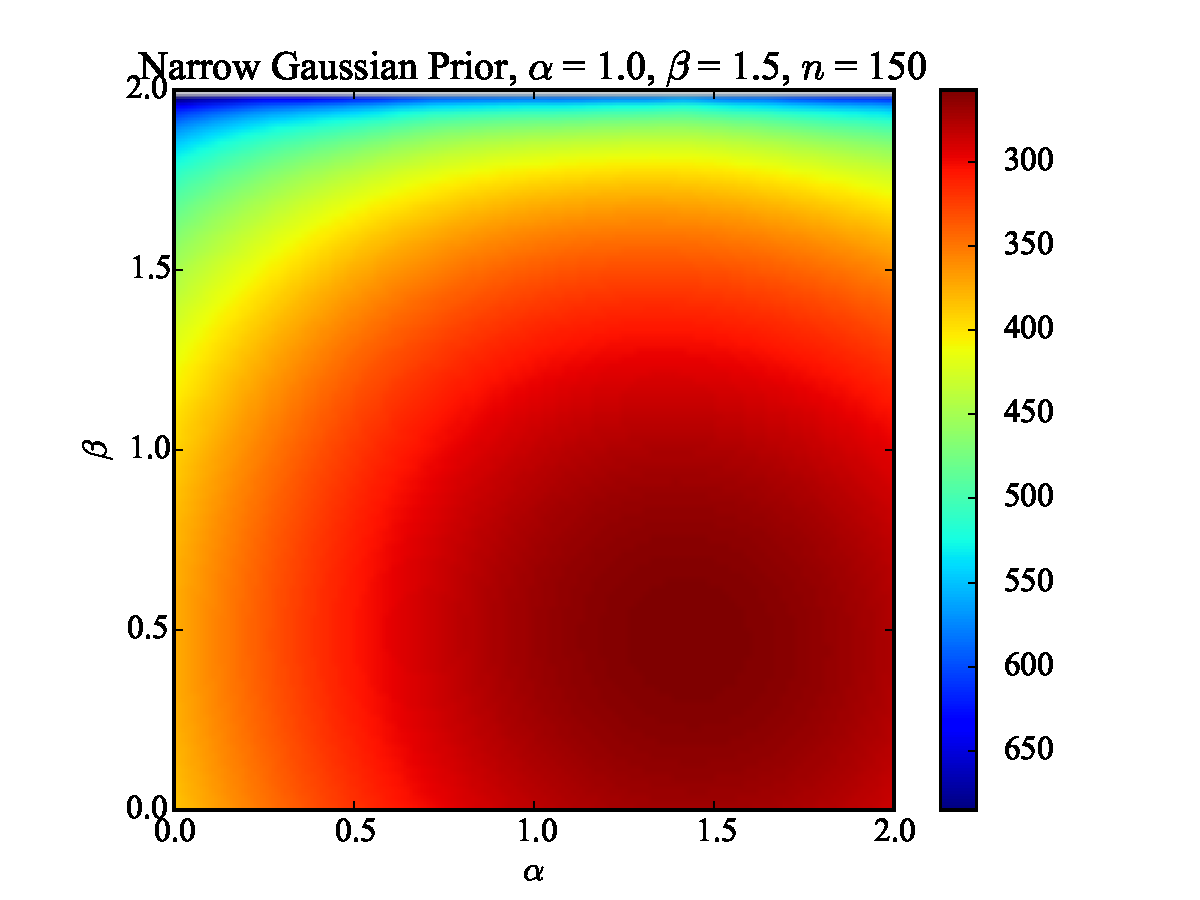
\includegraphics[width=0.49\textwidth]{lh2d_12.pdf}
    \caption{\label{2d_narrowgauss}Likelihoods for multiple $n$ with
    a narrow Gaussian prior.}
\end{figure}

\end{document}
